\section{Some results}

\subsection{Potential and charge distribution}

\begin{frame}{Charge distribution in 2D channel}
Thin channel, no flow, steady state:

\begin{figure}
\begin{center}
\includegraphics[width=0.9\textwidth]{../fig/charge_1d.pdf}
\end{center}
\caption{Computed positive (solid) and negative (dashed) charge
  distribution across a channel of width $d = 10 \mu$m. The solution
  in the channel is a KCl solution defined by parameters in table
  \ref{tab:res:param}. The channel walls are negatively charged.}
\label{fig:res:c_1d}
\end{figure}

\end{frame}

\subsection{Electroviscous effect}

\begin{frame}{Electroviscous effect in 2D channel}

Flow driven by a pressure gradient, walls of channel charged.

\begin{figure}
\begin{center}
\includegraphics[width=0.9\textwidth]{../fig/electrovisc.pdf}
\end{center}
\caption{Computed velocity profiles across a 2D channel of width $d =
  1 \mu$m. The flow is driven by a pressure gradient and the flow is
  slowed down due to the electroviscouos effect, this effects
  dependence on the surface charge $\sigma_s$ is here illustrated. The
  solution in the channel is a KCl solution defined by parameters in
  table \ref{tab:res:param}. In this simulation, $\sigma_0 = 0.89
  \mu$C/m$^2$, $\partial_xP = 1$ kPa/m and $u_0 = 10$ mm/s. }
\label{fig:res:ev}
\end{figure}
\end{frame}

\begin{frame}{Comparison with ``traditional'' approach}


\begin{figure}
\begin{center}
\includegraphics[width=0.9\textwidth]{../fig/electrovisc_comp.pdf}
\end{center}
\caption{Comparison between velocity profiles computed using a mean
  current (dotted) and by using the actual local current (dashed) for
  the streaming potential. The solution in the channel is a KCl
  solution defined by parameters in table \ref{tab:res:param}. In this
  simulation, $\sigma_0 = 0.89 \mu$C/m$^2$, $\partial_xP = 1$ kPa/m
  and $u_0 = 10$ mm/s. }
\label{fig:res:ev_comp}
\end{figure}

\end{frame}

\subsection{Flow through square array}

\begin{frame}{Flow through square array}

\begin{figure}
\begin{center}
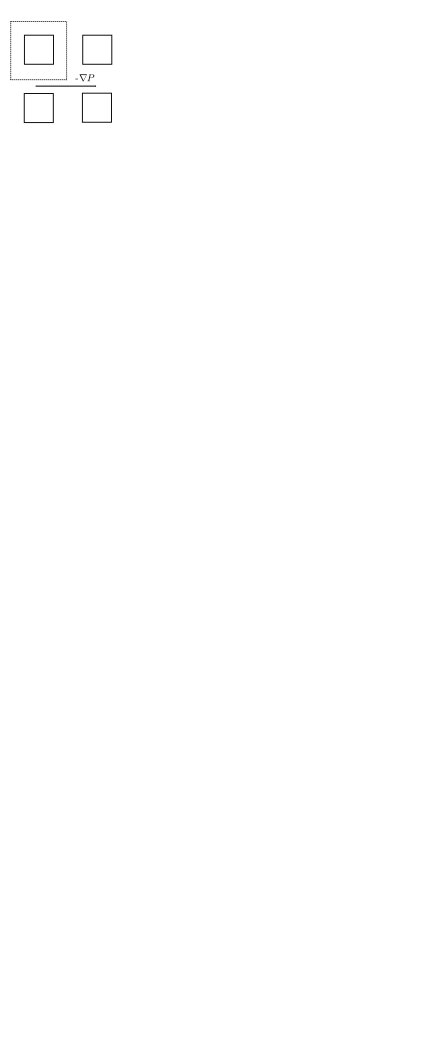
\includegraphics[width=0.7\textwidth]{../fig/square_setup.pdf}
\end{center}

\end{figure}

\end{frame}

\begin{frame}[plain]
\captionsetup[subfloat]{font=normalsize,
labelformat=empty,labelsep=space}

\begin{figure}
  \centering
  \subfloat{\label{fig:res:hedtasdro}\includegraphics[width=0.40\textwidth]{../fig/s_field_uncharged.pdf}}      
  \hspace{5pt}  \subfloat{\label{fig:resd:asas}\includegraphics[width=0.40\textwidth]{../fig/s_field_charged.pdf}}
\end{figure}

\vspace{-10pt}

\begin{figure}
  \centering
  \subfloat[$\;\;$ Uncharged
    ]{\label{fig:res:hetasddrdo}\includegraphics[width=0.40\textwidth]{../fig/s_u_uncharged.pdf}}      
  \hspace{5pt}  \subfloat[$\;\;$ Charged
    ]{\label{fig:res:asdas}\includegraphics[width=0.40\textwidth]{../fig/s_u_charged.pdf}}
\end{figure}

\end{frame}

\begin{frame}{Flow through square array}

\begin{figure}
\begin{center}
\includegraphics[width=0.9\textwidth]{../fig/square_u_mid.pdf}
\end{center}
\caption{Velocity profiles across the square array at $x = d/2$ in the
  cell. The sides of the squares are varied between $0.3d$, $0.5d$ and
  $0.7d$ where $d = 10 \mu$m is the length of the cell. The flow is
  driven by a pressure gradient and the uncharged (dashed) and charged
  (solid) squares are compared. In this simulation, $\sigma_s = 1.78
  \mu$C/m$^2$ (solid), $\partial_xP = 0.5$ kPa/m and $u_0 = 1$ mm/s. }
\label{fig:res:mid}
\end{figure}

\end{frame}

\subsection{A more complicated geometry}

\begin{frame}{A more complicated geometry}

\begin{figure}
  \centering
  \subfloat[$\;\;$ $|\ubf|$ Uncharged
    ]{\label{fig:res:hetasddrdo}\includegraphics[width=0.40\textwidth]{fig/u_uc.pdf}}      
  \hspace{5pt}  \subfloat[$\;\;$ $|\ubf|$ Charged
    ]{\label{fig:res:asdas}\includegraphics[width=0.40\textwidth]{fig/u_c.pdf}}
\end{figure}

\end{frame}


\begin{frame}{A more complicated geometry}

\begin{figure}
  \centering
  \subfloat[$\C_-$]{\label{fig:res:hedtasdro}\includegraphics[width=0.40\textwidth]{fig/cneg.pdf}}      
  \hspace{5pt}  \subfloat[$\C_+$]{\label{fig:resd:asas}\includegraphics[width=0.40\textwidth]{fig/cpos.pdf}}
\end{figure}

\end{frame}

\begin{frame}

\begin{center}
\Huge{Thanks for listening!}
\end{center}

\begin{center}
\Huge{Questions?}
\end{center}
\end{frame}
